\documentclass[12pt]{report}
\usepackage[a4paper]{geometry}
\usepackage[utf8]{inputenc}
\usepackage[english]{babel}
\usepackage[myheadings]{fullpage}
\usepackage[T1]{fontenc}
\usepackage{fancyhdr}
\usepackage{graphicx, setspace}
\usepackage{sectsty}
\usepackage{url}
\usepackage{amsthm}
\usepackage{amsmath}
\usepackage{mathtools}
\usepackage{amssymb}
\usepackage{bbm}
\usepackage{afterpage}
\usepackage{comment}
\usepackage{enumerate}
\usepackage{multirow}
\usepackage{float} %required for the placement specifier H
\usepackage{indentfirst}
\usepackage{yfonts}
\usepackage[ruled, vlined, portuguese]{algorithm2e}

\newtheorem{teorema}{Theorem}
\newtheorem{lema}[teorema]{Lemma}
\newtheorem{corolario}[teorema]{Corollary}
\newtheorem{proposicao}{Proposition}

\theoremstyle{definition}
\newtheorem{definicao}[teorema]{Definition}

\theoremstyle{remark}
\newtheorem{fato}[teorema]{Fact}
\newtheorem{demonstracao}{Proof}
\newtheorem{obs}{Remark}
\newtheorem{propriedades}{Properties}

\newcommand{\R}{\mathbb{R}}
\newcommand{\Q}{\mathbb{Q}}
\newcommand{\Z}{\mathbb{Z}}
\newcommand{\N}{\mathbb{N}}
\newcommand{\C}{\mathbb{C}}
\newcommand{\Hi}{\mathbb{H}}
\newcommand\restr[2]{{% we make the whole thing an ordinary symbol
  \left.\kern-\nulldelimiterspace % automatically resize the bar with \right
  #1 % the function
  \vphantom{\big|} % pretend it's a little taller at normal size
  \right|_{#2} % this is the delimiter
  }}


\DeclareMathOperator{\famcirc}{C}
\DeclareMathOperator{\TLF}{TLF}
\DeclareMathOperator{\T}{T}
\DeclareMathOperator{\ST}{ST}
\DeclareMathOperator{\TS}{TS}
\DeclareMathOperator{\capacidade}{cap}
\DeclareMathOperator{\valor}{val}
\DeclareMathOperator{\mdc}{mdc}
\DeclareMathOperator{\adj}{adj}
\DeclareMathOperator{\gr}{gr}



%%------ 
%% Comandos gerais
%% Observação: o arquivo "comandos.tex" tem que estar presente.
%%------
%%%%%%%%%%%%%%%%%%%%%%%%%%%%%%%%%%%%%%%%%%%%%%%%%%%%%%%%%%%%%%%%%%%%%
% In English:
%    This is a list of commands specification for FAPESP reports.
%
% In Portuguese:
%    Esta é uma lista de especificação de comandos para relatórios
% da Fundação de Amparo à pesquisa do Estado de São Paulo (FAPESP).
%
% Author/Autor: André Leon Sampaio Gradvohl, Dr.
% Email:        andre.gradvohl@gmail.com
% Lattes CV:    http://lattes.cnpq.br/9343261628675642
% 
% Last update/Última versão: 11/Sep/2016
%%%%%%%%%%%%%%%%%%%%%%%%%%%%%%%%%%%%%%%%%%%%%%%%%%%%%%%%%%%%%%%%%%%%%%

\newcommand{\HRule}[1]{\rule{\linewidth}{#1}}
\setcounter{tocdepth}{3}
\setcounter{secnumdepth}{3}

\newcommand{\titulo}[1]{\def\meuTitulo{#1}}
\newcommand{\tituloIngles}[1]{\def\meuTituloIngles{#1}}
\newcommand{\numProjeto}[1]{\def\numFAP{#1}}
\newcommand{\tipoRelatorio}[1]{\def\tipoRelat{#1 }} %o espaço depois do #1 é importante
\newcommand{\modalidadeProjeto}[1]{\def\modProjeto{#1}} 
\newcommand{\agFomento}[2]{\def\agFom{#1} \def\siglaAgFom{#2}} %extenso Sigla
\newcommand{\autor}[1]{\def\nomeAutor{#1}}
\newcommand{\cidade}[1]{\def\nomeCidade{#1}}
\newcommand{\universidade}[1]{\def\nomeUniversidade{#1}}
\newcommand{\faculdade}[1]{\def\nomeFaculdade{#1}}
\newcommand{\periodoVigencia}[1]{\def\periodVig{#1}}
\newcommand{\periodoRelatorio}[1]{\def\periodRelat{#1}}

\author{}
\date{}

%Definição de membros da equipe de pesquisas
\newcommand{\membroA}[1]{\def\nomeMembroA{#1}}
\newcommand{\membroB}[1]{\def\nomeMembroB{#1}}
\newcommand{\membroC}[1]{\def\nomeMembroC{#1}}
\newcommand{\membroD}[1]{\def\nomeMembroD{#1}}
\newcommand{\membroE}[1]{\def\nomeMembroE{#1}}
\newcommand{\membroF}[1]{\def\nomeMembroF{#1}}

\newcommand{\Figure}[1]{Figura~\ref{fig:#1}}
\newcommand{\Table}[1] {Tabela~\ref{#1}}
\newcommand{\Equation}[1] {Equa\c{c}\~ao~\ref{#1}}
\newcommand{\addFigure}[3] { %Parametros scale, fig_name, caption 
    \begin{figure}[!hbt]
      \centering
      \includegraphics[scale=#1]{figures/}
      \caption{#3}\label{fig:#2}
    \end{figure}
}

\newcommand{\geraTitulo}{
\clearpage
\begin{titlepage}
  \begin{center}
      \vspace*{-3cm}
       { \setstretch{.5} 
         \textsc{\nomeUniversidade} \\
         \HRule{.2pt}\\
         \textsc{\nomeFaculdade}
       }

       \vspace{5.5cm}

       \Large \textbf{\textsc{\meuTitulo}}
 	  \HRule{1.5pt} \\ [0.5cm]
       \linespread{1}
       %\large Scientific Report 
       \ifdefined\tipoRelat
            \tipoRelat
       \fi
       \large Scientific Report 
       of the project 
       \ifdefined\modProjeto
           in the \modProjeto
       \fi
       \hspace{.01} mode, financed by \agFom. \\ 
   	   \HRule{1.5pt} \\ [0.5cm]

       \ifdefined\numFAP
          Project \siglaAgFom~\texttt{\#\numFAP}
          \\ [0.5cm]
       \fi
        Alumna : \nomeAutor
        \\
        Researcher in charge : \nomeMembroA
       
        \vfill
       
        {\normalsize  \nomeCidade, \today}
 \end{center}
 \end{titlepage}
}

\usepackage{titlesec}
\titleformat{\chapter}{\normalfont\LARGE\bfseries}{\thechapter}{1em}{}
\titlespacing*{\chapter}{0pt}{3.5ex plus 1ex minus .2ex}{2.3ex plus .2ex}

%----------------------------------------------------------------------
% Cabeçalho e rodapé
%----------------------------------------------------------------------
\pagestyle{fancy}
\fancyhf{} % Limpa todos os campos de header and footer fields
\renewcommand{\headrulewidth}{0pt}
\fancyfoot[R]{\thepage}

\addto\captionsportuguese{\renewcommand{\contentsname}{Summary}}
\addto\captionsportuguese{\renewcommand{\bibname}{References}}

%------
% Resumo e Abstract
%------
\newcommand{\Resumo}[1]{
   \begin{otherlanguage}{portuguese}
       \addcontentsline{toc}{chapter}{Resumo}
       \begin{abstract} \thispagestyle{plain} \setcounter{page}{2}
          #1
        \end{abstract}
   \end{otherlanguage} 
} %end \Resumo

\newcommand{\Abstract}[1]{
   \begin{otherlanguage}{english}
      \addcontentsline{toc}{chapter}{Abstract}
      \begin{abstract} \thispagestyle{plain} \setcounter{page}{3}
       #1
      \end{abstract}    
    \end{otherlanguage} 
} %end \abstract

%------
% Folha de rosto
%------
\newcommand{\folhaDeRosto}{
   \chapter*{General Project Information}
   \addcontentsline{toc}{chapter}{General Project Information}
   \begin{itemize}
      \item Title: 
            \begin{itemize}\item[] \textbf{\meuTitulo} \end{itemize}
      \item Author: 
            \begin{itemize}\item[]\textbf{\nomeAutor}\end{itemize}
      \item Institution of the project: 
            \begin{itemize}
               \item[]\textbf{\nomeFaculdade \ da \nomeUniversidade} 
            \end{itemize}
      \item Researcher in charge:
            \begin{itemize}
               \ifdefined\nomeMembroA
                 \item[]\textbf{\nomeMembroA}
               \else 
                 \item[]\textbf{\nomeAutor}
               \fi
               \ifx\nomeMembroB\undefined\else \item[]\textbf{\nomeMembroB}\fi
               \ifx\nomeMembroC\undefined\else \item[]\textbf{\nomeMembroC}\fi
               \ifx\nomeMembroD\undefined\else \item[]\textbf{\nomeMembroD}\fi
               \ifx\nomeMembroE\undefined\else \item[]\textbf{\nomeMembroE}\fi
               \ifx\nomeMembroF\undefined\else \item[]\textbf{\nomeMembroF}\fi
             \end{itemize}
       
          \ifdefined \numFAP
             \item Number of the research project:
             \begin{itemize}
                 \item[]\textbf{\numFAP} 
             \end{itemize}
          \fi  
       \item Duration:
            \begin{itemize}
               \item[]\textbf{\periodRelat} 
            \end{itemize}
       \item Period covered by this research report:
            \begin{itemize}
               \item[]\textbf{\periodVig} 
            \end{itemize}
   \end{itemize}
   \clearpage
}
%
%%-----
%% Página de título
%% Observação: As definições que aparecem a seguir comporão a
%%             página de título e a folha de rosto.
%%-----
%% Define o nome da universidade onde o projeto foi desenvolvido.
\universidade{University of São Paulo}
%
%% Define o nome da faculdade onde o projeto foi desenvolvido.
\faculdade{Institute of Mathematics and Statistics (IME)}
%
%% Define o título do projeto.
\titulo{TOPOLOGY AND GEOMETRY OF 3-MANIFOLDS}
%
%% Define a agencia de Fomento e a abreviatura. O primeiro argumento é o 
%% nome por extenso e o segundo a abreviatura.
%% Ambos os argumentos são obrigatórios
\agFomento{Fundação de Amparo à Pesquisa do Estado de São Paulo}{FAPESP}
%
%% Define o tipo de relatório. Pode ser Anual ou Final.
%% Não é obrigatório definir o tipo de relatório.
\tipoRelatorio{Annual}
%
%% Define a modalidade de Projeto. Pode ser temático, regular, etc.
\modalidadeProjeto{Thematic Research Assistance - Scientific Initiation}
%
%% Define o número do projeto.
%% Não é obrigatório definir o número do projeto.
\numProjeto{2021/06678-5} 
%
%% Define o autor do relatório.
\autor{Isabela Miki Suzuki}
%
%% Define a equipe do projeto (incluindo o pesquisador responsável no comando \membroA{}
\membroA{André Salles de Carvalho}
%% Define o período da vigência do Projeto.
\periodoRelatorio{01/08/2021 to 31/07/2023}
%
%% Define o período coberto pelo relatório.
\periodoVigencia{01/08/2021 to 31/07/2022}
%
%% Define a cidade onde o projeto foi desenvolvido.
\cidade{Itapecerica da Serra}

%%-----
%% Página de título
%% Observação: Os comandos a seguir não devem ser mudados, 
%%             exceto caso necessário.
%%-----
\begin{document}
%
%% Define a numeração em romanos.
\pagenumbering{roman}
%
%% Gera a folha de título.
\geraTitulo
%
%% Gera a folha de rosto.
\folhaDeRosto
%
%% Escreva aqui o resumo em português.
%\Resumo{
%Isso é um teste babalsbak das bsak blkab lsab dbaslkb saldbd lsab %lasbdlsba ldbsa lbds lab ldkasbkldbs alk bdaslkb ldsakb lsdablk bald %blkb dlskab lasdbl sablkds ablkb lkasbd lsdbaklb d 
%  }
%
%% Escreva aqui o resumo em inglês.
%\Abstract{
%teste in english
%}
%
%% Adicionará o sumário.
%% Mantenha o \thispagestyle{empty} e \clearpage
\tableofcontents
\thispagestyle{empty}
\clearpage
%
%% Define a numeração em arábicos.
\pagenumbering{arabic}

%%-----
%% Formatação do título da seção
%%-----
\sectionfont{\scshape}

%%-----
%% Corpo do texto
%%-----
\chapter{Summary of the proposed project}\label{chp:resumoProj} 

This project aims to study the topology and geometry of 3-manifolds and is based on the notes  \cite{Andre} "Topologia e Geometria de 3-variedades: Uma Agradável Introdução" ("Topology and Geometry of 3-manifolds: A Pleasant Introduction"), prepared by the advisor of this project in collaboration with Rafał Siejakowski, from IME-USP, to follow an introductory course of the same title at the 33rd Brazilian Mathematics Colloquium. Topics to be discussed include inversive geometry, the 3-sphere, and an introduction to geometric manifolds and structures in 2- and 3-manifolds.

\chapter{Summary of the activities}\label{chp:resumoAtiv}

In this project, we focused on the 3-sphere, an important 3-manifold, and were able to study it as a one-point compactification, subset of the quaternions, matrix group, union of disjoint circles, and as an union of "concentric" tori. For all that, it is necessary to know about inversions and möbius transformations, and that's how we will begin this report.

The main references were \cite{Andre}"Topologia e geometria de 3-variedades - Uma agradável introdução", from Carvalho and Siejakowski for the various aspects of the 3-sphere, \cite{Ahlfors} "Complex Analysis An Introduction to the Theory of Analytic Functions of One Complex Variable", from Ahlfors for the möbius transformations study and \cite{Coxeter} "Introduction to geometry", from Coxeter for Villarceau circles. More informations about these books can be found by the end of this document.
%, as two solid toruses and as a Lie group.

\chapter{Project execution}\label{chp:realizacoes}

\section{Inversion}\label{inver}

\begin{definicao}[Inversion]
Let S $\subset \R^{n+1}$ be the sphere of center O and radius 1, the inversion in S, denoted by $\iota_S : \R^{n+1}\setminus{\{O\}} \rightarrow \R^{n+1}\setminus{\{O\}}$, is defined by $\iota_S (P) = P^*$, where P$^*$ is the point on the radius with origin in O and that passes through P such that $|OP| \cdot |OP^*| = r^2$.
\end{definicao}

\begin{figure}[H]
    \centering
    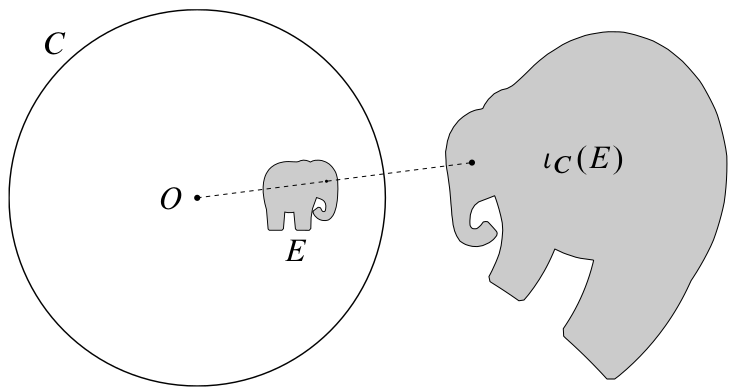
\includegraphics[scale=0.35]{inversao.png}
    \caption{Inversion in $\R^2$}
    \label{fig:5}
\end{figure}

Inversions have the following properties:
\begin{itemize}
    \item $\iota_S$ has order 2, i.e., $\iota_S \circ \iota_S = Id$;
    \item $\iota_S$ fixes any point on C;
    \item $\iota_S$ changes the parts of the plane that are inside and outside C;\\
    $\left(\mbox{Proof: }|OP|<r \Rightarrow |OP*|=\frac{r^2}{|OP|} > r \mbox{ since }|OP|<r\right)$
    \item ($k \leq n$) $\iota_S$ carries k-spheres into k-spheres (remembering that k-planes are k-spheres - they are the ones with $\infty$ radius);
    \item ($k \leq n$) If $S'$ is a k-sphere that contains the center of $S$, then, $\iota_S[S']$ is a k-plane;
    \item $\iota_S$ is a conformal map, i.e., preserves angles between curves;
    \item Considering the isomorphism $\R^2 \cong \C$, if $C$ is the circle of radius 1 and center on $0$, then $\iota_C(z) = \frac{1}{\hat{z}}$ $\left( \mbox{because } z=re^{i\theta}, \frac{1}{\bar{z}} = \frac{1}{re^{-i\theta}} = \frac{e^{i\theta}}{r} = \frac{z}{r^2}\right)$
\end{itemize}

\section{Möbius transformation}\label{TLF} %\cite{Ahlfors}
\subsection{The linear group}

\begin{definicao} The group of linear fractional transformations is defined by
\begin{equation*}
\TLF \doteq \left\{ T:\hat{\C}\rightarrow\hat{\C}\text{; }T(z)=Tz=\frac{az+b}{cz+d}\text{ : }a,b,c,d \in \C\text{; }ad-bc\neq0\text{; }T\infty=\frac{a}{c}\text{; }T(-\frac{d}{c})=\infty \right\}
\end{equation*}
With the composition ($\circ$) operator.\\
T $\in \TLF$ \text{ is called (fractionary) linear transformation or Möbius transformation.}
\end{definicao}

\begin{obs}
It is common to have a $\hat{\C}$ together with $\TLF$, but for technical reasons we will omit it.
\end{obs}

\begin{definicao}
Being
\begin{equation*}
N = \left\{ \alpha I \in \operatorname{M}_{2x2}(\C) : \alpha \in \R^* \right\}
\end{equation*}
The projective special linear group is defined by 
\begin{equation*}
\operatorname{PSL}(2, \C) \doteq \left\{ A = \begin{bmatrix}
a & b\\
c & d
\end{bmatrix} : a,b,c,d \in \C\text{; }det(A)\neq0 \right\} \Bigg/ N
\end{equation*}
with the matrices product operator.
\end{definicao}

\begin{teorema}
We have
\begin{equation*}
(\TLF, \cdot) \cong (\operatorname{PSL}(2, \C), \circ)
\end{equation*}
\text{And the proof is trivial.}
\end{teorema}

Note here that $Tz = \frac{1}{z}$ $\in \TLF$ is a inversion considering the isomorphism $\C \cong \R^2$.

If $c\neq0:$
\begin{gather*}
    \frac{az+b}{cz+d} = \frac{bc-ad}{c^2(z+\frac{d}{c})} + \frac{a}{c}
\end{gather*}
which is a composition of a conjugation, with a translation, an inversion, a rotation, and a homothetic transformation followed by another translation.

If $c=0:$
\begin{gather*}
    \frac{a}{d}z + \frac{b}{d}
\end{gather*}
is a translation followed by rotation and homothetic transformation.

\begin{fato}
\text{Any linear transformation that preserves the real axis can be written with only}\\
\text{real coefficients.}
\end{fato}

%demonstração??

\subsection{Cross ratio} \label{cross}
\begin{definicao}
The cross ratio (z$_1$, z$_2$, z$_3$, z$_4$), with z$_1$, z$_2$, z$_3$, z$_4$ $\in \hat{\C}$ is the image of $z_1$\\
by the linear transformation that carries z$_2$, z$_3$, z$_4$ to 1, 0, $\infty$, in this order.\\
z$_2$, z$_3$, z$_4$ must be distinct because linear transformations are injective.
\end{definicao}

\begin{fato}
Calling S the linear transformation cited above:\\
If z$_2$, z$_3$, z$_4$ $\in \C$:\\
\begin{equation*}
    \operatorname{S}z=\frac{z-z_3}{z-z_4} \cdot \frac{z_2-z_4}{z_2-z_3}
\end{equation*}
If z$_2$, z$_3$ or z$_4$ = $\infty$:\\
\begin{equation*}
    \operatorname{S}z = \frac{z - z_3}{z - z_4} \text{, } \operatorname{S}z = \frac{z_2 - z_4}{z - z_4} \text{, } \operatorname{S}z = \frac{z - z_3}{z_2 - z_3}
\end{equation*}
respectively.
\end{fato}

\begin{fato}
The cross ratio is well defined, i.e., for distinct z$_2$, z$_3$, z$_4$ $\in \hat{\C}$, that is only one linear transformation that carries z$_2$, z$_3$, z$_4$ to 1, 0, $\infty$.
\end{fato}

\begin{proof}
Fix distinct z$_2$, z$_3$, z$_4$ $\in \hat{\C}$ and suppose that S and T $\in$ $\TLF$ carries, respectively z$_2$, z$_3$, z$_4$ to 1, 0, $\infty$.\\
Since ($\TLF$, $\circ$) is a group, $\ST^{-1}$ $\in$ $\TLF$, so that is a, b, c, d $\in \C$ such that
\begin{equation*}
    \ST^{-1}(z) = \frac{az+b}{cz+d}
\end{equation*}
 and since 
 \begin{equation*}
    \ST^{-1}(1) = \frac{a+b}{c+d} = 1;\text{ } \ST^{-1}(0) = \frac{b}{d} = 0;\text{ } \ST^{-1}(\infty) = \frac{a\infty+b}{c\infty+d} = \infty
 \end{equation*}
we have a + b = c + d, b = 0, c = 0, d $\neq \infty$.\\ 
So b = c = 0 and a = d $\neq \infty$, and therefore, $\ST^{-1} = Id$ (identity).
\end{proof}

\begin{teorema}
If T $\in$ $\TLF$, (Tz$_1$, Tz$_2$, Tz$_3$, Tz$_4$) = (z$_1$, z$_2$, z$_3$, z$_4$).
\end{teorema}

\begin{teorema}
(z$_1$, z$_2$, z$_3$, z$_4$) $\in$ $\R$ $\Leftrightarrow$ z$_1$, z$_2$, z$_3$, z$_4$ are in the same circle.
\end{teorema}

\begin{corolario}
Linear transformations carry circles into circles.
\end{corolario}

\begin{fato}
For any z$_2$, z$_3$, z$_4$ $\in$ $\hat{\C}$, distincts, and a$_2$, a$_3$, a$_4$ $\in$ $\hat{\C}$ distincts; there is a linear transformation carrying z$_2$, z$_3$, z$_4$ to a$_2$, a$_3$, a$_4$ in this order.

For that, find the linear transformations that carries z$_2$, z$_3$, z$_4$ into 1, 0, $\infty$ (let's call this one T) and a$_2$, a$_3$, a$_4$ into 1, 0, $\infty$ (this one will be S) and take S$^{-1}$T $\in$ $\TLF$.
\end{fato}

\begin{fato}
In face of the last fact, for any two circles (remembering that lines are circles) that is a linear transformation carrying one to another.

For that, fix 3 points in each circle, apply the last fact and note that for 3 points there is only one circle passing for them and that linear transformations carry circles into circles.
\end{fato}

\subsection{Symmetry}

\begin{definicao}
Let C be a circle on the complex plane, and z$_1$, z$_2$, z$_3$ $\in$ C distincts. The points z, z$^{*}$ $\in \hat{\C}$  are said to be symmetric in relation to C if
\begin{equation*}(z^{*}, z_1, z_2, z_3) = \overline{(z, z_1, z_2, z_3)}.
\end{equation*}
\end{definicao}

\begin{obs}
Fix a circle C; arbitrary distincts points w$_1$, w$_2$, w$_3$ $\in$ C; w, w$^{*}$ $\in$ $\hat{\C}$ and a linear transformation S that carries the real axis into C such that there are distincts a$_1$, a$_2$, a$_3$ $\in \R$ : Sa$_1$=w$_1$, Sa$_2$=w$_2$, Sa$_3$=w$_3$.
\begin{equation*}
    (w^{*}, w_1, w_2, w_3) = \overline{(w, w_1, w_2, w_3)}\Leftrightarrow
\end{equation*}    
%\text{ and since } ($\TLF$, \circ) \text{ is a group, we know that that is }S^{-1} \in $\TLF$, \text{ so we }
\begin{equation*}
    \frac{S^{-1}w^{*}-a_2}{S^{-1}w^{*}-a_3} \cdot \frac{a_1-a_3}{a_1-a_2} = (S^{-1}w^{*}, a_1, a_2, a_3) = \overline{(S^{-1}w, a_1, a_2, a_3)} = \overline{\left(\frac{S^{-1}w-a_2}{S^{-1}w-a_3} \cdot \frac{a_1-a_3}{a_1-a_2}\right)} =
\end{equation*}
\begin{equation*}
    \frac{\overline{S^{-1}w}-a_2}{\overline{S^{-1}w}-a_3} \cdot \frac{a_1-a_3}{a_1-a_2} \Leftrightarrow
\end{equation*}
\begin{equation*}
    \overline{S^{-1}w} = S^{-1}w^{*} \Leftrightarrow    
\end{equation*}
If T is a linear transformation carrying the real axis into C; there are z, z$^{*}$ $\in$ $\hat{\C}$ such that Tz$^*$ = w$^*$ and Tz = w; and $\ST^{-1}$ carries the real axis into itself, then it can be written with only real coefficients, so by the properties of conjugate,
\begin{equation*}
    S^{-1}Tz^{*} = S^{-1}w^{*} = \overline{S^{-1}w} = \overline{S^{-1}Tz} = S^{-1}T\bar{z}
\Leftrightarrow 
\end{equation*}
If T $\in$ $\TLF$ carries the real axis into C and z into w, then carries $\bar{z}$ into w$^{*}$.
\end{obs}

\BlankLine

Directly arrising from that last remark, we have the following properties:
\begin{itemize}
    \item Just the points on C are symmetric to themselves.
    \item The map that carries z to $z^{*}$ is an inversion. [See section \ref{inver}]
    \item Two inversions compposed result in a linear transformation.
\end{itemize}

\begin{teorema} (The symmetry principle)\\
If a linear transformation carries a circle C$_1$ into a circle C$_2$, then it transforms any C$_1$-symmetric pair of points into a C$_2$-symmetric pair.
\end{teorema}

\subsection{Families of circles}
For this study, we will begin fixing a linear transformation:
\begin{gather*}
    \operatorname{T}:\hat{\C} \rightarrow \hat{\C}\\
    \operatorname{T}z = k \frac{z - a}{z - b}
\end{gather*}
$a, b, k$ $\in \C$; $a$ $\neq$ $b$

It is easy to see that a circle that passes through $a$ and $b$ is carried by T to a line that passes through 0 and $\infty$ and that each circle defined by the equation, $\rho \in \R$:

\begin{gather*}
    \frac{|z-a|}{|z-b|} = \frac{\rho}{|k|}
\end{gather*}
will be carried to the circle with center in 0 and radius $\rho$.

Since T $\in$ $\TLF$ is a bijection, the pre-image by T of all the lines that pass through 0 and $\infty$, which union results in the entire plane, is the set of all the circles that pass through $a$ and $b$ (we'll call it C$_1$), with union resulting also in the whole plane. Besides that, the pre-image by T of all the circles centered in 0, that, united with \{ $a, b$ \}, covers the plane completely is the set of all the circles that have fixed ratio of the distance to $a$ by the distance to $b$ (we'll call it C$_2$, and these circles are called Apollonian circles), which also covers the entire plane with the exception of the points $a$ and $b$.

\begin{figure}[H]
    \centering
    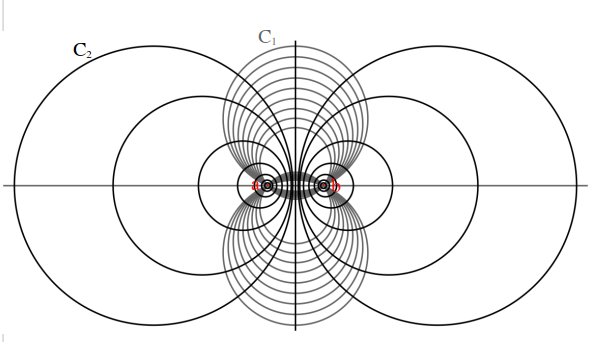
\includegraphics[scale=0.35]{steiner.png}
    \caption{C$_1$ and C$_2$, which together form the denominated circular net or Steiner circles.}
    \label{fig:steiner}
\end{figure}

These families present the following properties:
\begin{itemize}
    \item In the plane, for each point that is not $a$ nor $b$, passes one circle from C$_1$ and another from C$_2$;
    \item $\alpha_1 \perp \alpha_2, \forall \alpha_1 \in$ C$_1,  \alpha_2 \in$ C$_2$;
    \item $\forall \hat{\alpha}_1 \neq \alpha_1 \in$ C$_1$, $\hat{\alpha}_2 \neq \alpha_2 \in $C$_2$,
    \begin{equation*}
    \iota_{\alpha_1}[\alpha_2] = \alpha_2,\text{  } \iota_{\alpha_2}[\alpha_1] = \alpha_1, \text{  } \iota_{\alpha_1}[\hat{\alpha}_1] \in \operatorname{C}_1\setminus{\{\hat{\alpha}_1\}}, \text{  } \iota_{\alpha_2}[\hat{\alpha}_2] \in \operatorname{C}_2\setminus{\{\hat{\alpha}_2\}}
    \end{equation*}
    \item $a$ and $b$ are symmetric only in relation to the circles of C$_2$.
\end{itemize}

\subsubsection{Linear transformations between families of circles}

If T $\in$ $\TLF$ carries $a$ to $a$' and $b$ to $b$', because of [section \ref{cross}], that is $k \in \C$ such that

\begin{gather*}
    \frac{\operatorname{T}z-a'}{\operatorname{T}z-b'} = k \frac{z-a}{z-b}, \forall z \in \hat{\C}
\end{gather*}

It is clear that T carries C$_1$ and C$_2$ respectively into C'$_1$ and C'$_2$, the Steiner circles with foci $a$ and $b$ and $a$' and $b$', in order.

If $a' = a$ and $b' = b$, $a$ and $b$ are called fixed points of T and stay convenient represent z and Tz on the same plane.

Under these circumstances, the whole circular net is mapped into itself.

The value of $k$ serves to identify the image cicles C'$_1$ and C'$_2$. In fact, with appropriate orientation, $\forall \alpha_1 \in$ C$_1$, the angle between $\alpha_1$ and $T[\alpha_1]$ is $arg(k)$, and obviously
\begin{equation*}
    \frac{\frac{|\operatorname{T}z-a|}{|\operatorname{T}z-b|}}{\frac{|z-a|}{|z-b|}} = |k|, \forall z \in \alpha_2, \forall \alpha_2 \in \famcirc_2,
\end{equation*}
i.e., the quocient of the constant ratios of each circle in C$_2$ and their images are given by $k$.

The special cases in which 
\begin{equation*}
    \operatorname{T}[\alpha_1]=\alpha_1, \forall \alpha_1 \in \famcirc_1
\end{equation*}
or
\begin{equation*}
\operatorname{T}[\alpha_2]=\alpha_2, \forall \alpha_2 \in \famcirc_2    
\end{equation*}
are particularly important.

The first case occurs when $k>0$ and the linear transformation will be called hiperbolic. And the other, in which T will be called elliptic, occurs when $|k|=1$.

\begin{proposicao}
Let $\operatorname{g} : S^2 \rightarrow \hat{\C}$ be a stereographic projection [See section \ref{projest}] (considering the isomorphism $\R^2 \cong \C$).\\
Then \\
$R : S^2 \rightarrow S^2$ is a rotation on $S^2$ $\Leftrightarrow \operatorname{g} \circ R \circ \operatorname{g}^{-1}$ is elliptic and has two fixed points: $a$ and $-\frac{1}{a}$, with $a \in \hat{\C}$
\end{proposicao}

\begin{obs}
It means that the image of parallel circles on S$^2$ by stereographic projection will be Apollonian circles on $\R^2 \cong \C$.
[Proof in appendix - proof \ref{proofRemark3}]
\end{obs}

%%%%%%%%%%%%%%%%%%%%%%%%%%%%%%%%%%%%%%%%%%%%%%%%%%%%%%%%%%%%%%%%%%%%%
%    proof 1
%%%%%%%%%%%%%%%%%%%%%%%%%%%%%%%%%%%%%%%%%%%%%%%%%%%%%%%%%%%%%%%%%%%%%

%This project consisted of a detailed study of 3-sphere isomorphisms, an important 3-manifold.

%O projeto consistiu no estudo detalhado de isomorfismos da 3-esfera, uma importante 3-variedade.\hfill \break

\section{Spheres}

Here we start our discussion about the 3-sphere, and for that, we declare now its general definition.

\begin{definicao}[n-sphere]
The n-sphere, $n \in \N$,  S$^n$ is the subset of $\R^n$ with points that have a distance 1 from the origin, i.e.,
\begin{equation*}
    S^{n} = \{x \in \R^{n} : || x || = 1\}
\end{equation*}
\end{definicao}

\section{3-sphere is a 3-manifold}

\begin{definicao}[Topological n-manifold]
A (topological) n-manifold is a Hausdorff topological space M with an enumerable basis such that $\forall$ p $\in$ M there is a neighborhood U of p homeomorphic to an open set in $\R^n$
\end{definicao}

We won't prove it because it is out of our scope, but it is well known that S$^3$ is a Hausdorff topological space with an enumerable basis. The second part of the requirements will be clear by the end of the next section.

\section{3-sphere as one-point compactification of $\R^3$}
S$^3$ is homeomorphic to $\hat{\R}^3$ and this homeomorphism is given by the stereographic projection g, which is an extension of a restriction of an inversion.

\subsection{General case} \label{projest}
In the general case, with $\vec{x} \in \R^{n}$ and $t \in \R$, we have:

\begin{gather*}
\operatorname{g} : S^n \rightarrow \hat{\R}^n \\
\operatorname{g}(\vec{x}, t) =
    \begin{cases}
        \infty, \text{ if }\vec{x} = 0, t = 1 \\
        \frac{1}{1 - t} \vec{x}, \mbox{ } c.c.
    \end{cases}
\end{gather*}

And g is a homeomorphism. [Proof in appendix - proof \ref{proofghomeo}]

%%%%%%%%%%%%%%%%%%%%%%%%%%%%%%%%%%%%%%%%%%%%%%%%%%%%%%%%%%%%%%%%%%%%%%% proof
%%%%%%%%%%%%%%%%%%%%%%%%%%%%%%%%%%%%%%%%%%%%%%%%%%%%%%%%%%%%%%%%%%%%%%

\subsection{Stereographic projection and inversion}

In $\R^{n+1}$, let S be the sphere with center $(0, ..., 0, 1)$ and radius $\sqrt{2}$\\
And let's consider the inversion in $S$, which can be given by the formula:
%(it is easy noting that $\iota_{S}$ is the composition ):

\begin{equation*}
    \iota_{S}(x_1, ..., x_n, t) = \left( \frac{2(x_1, ..., x_n)}{||(x_1, ..., x_n)||^2 + (t-1)^2}, \frac{2(t-1)}{||(x_1, ..., x_n)||^2 + (t-1)^2} + 1 \right)
\end{equation*}

Since S$^n$ contains the center of S, $\iota_s[S^n]$ is a n-plane [See section \ref{inver}].

In fact, we have:

\begin{equation*}
    \forall (x_1, ..., x_n, t) \in S^n \Rightarrow ||(x_1, ..., x_n)||^2+t^2=1
\end{equation*}

\begin{equation*}
    \iota_{S}(x_1, ..., x_n, t) = \left( \frac{2(x_1, ..., x_n)}{||(x_1, ..., x_n)||^2 + (t-1)^2}, \frac{2(t-1)}{||(x_1, ..., x_n)||^2 + (t-1)^2} + 1 \right) =
\end{equation*}

\begin{equation*}
    \left( \frac{(x_1, ..., x_n)}{1-t}, \frac{2t-2}{2-2t}+1 \right) = \left( \frac{(x_1, ..., x_n)}{1-t}, 0 \right)
\end{equation*}

So,

\begin{gather*}
\operatorname{g} : S^n \rightarrow \hat{\R}^n \\
\operatorname{g}(\vec{x}, t) =
    \begin{cases}
        \infty, \text{ if }\vec{x} = 0, t = 1 \\
        \frac{1}{1 - t} \vec{x} \cong \iota_{S}(\vec{x}, t), \mbox{ } c.c.
    \end{cases}
\end{gather*}

%\subsection{2-sphere case}
%
%\begin{equation*}
%g : S^2 \rightarrow \hat{\R}^2 \\
%\end{equation*}
%\begin{align*}
%g(0, 0, 1) = \infty \\
%g(x_1, x_2, t) = \frac{1}{1 - t} \cdot (x_1, x_2) \\
%\end{align*}
%
%Since $\R^2 \cong \C$ and 
%
%\begin{equation*}
%g : S^2 \rightarrow \hat{\R}^2 \\
%\end{equation*}
%\begin{align*}
%g(0, 0, 1) = \infty \\
%g(x_1, x_2, t) = \frac{1}{1 - t} \cdot (x_1, x_2) \\
%\end{align*}
%

\subsection{3-sphere case}

\begin{gather*}
\operatorname{g} : S^3 \rightarrow \hat{\R}^3 \\
\operatorname{g}(x_1, x_2, x_3, t) =
    \begin{cases}
        \infty,\text{ if } x_1 = x_2 = x_3 = 0, t = 1 \\
        \frac{1}{1 - t} (x_1, x_2, x_3), \text{ } c.c.
    \end{cases}
\end{gather*}

With that, g is the homeomorphism between S$^3$ and $\hat{\R}^3$.

Knowing that is a Hausdorff topological space with an enumerable basis, it is clear now that S$^3$ is a 3-manifold.

\subsection{1-sphere case}
The 1-sphere case, however, has an easier approach.

For each point P or Q in the 1-sphere, we can define 
\begin{align*}
    \operatorname{g}(0, 1) = \infty\mbox{, }\operatorname{g}(P) = P^*\mbox{ and }\operatorname{g}(Q) = Q^* 
\end{align*}
as the figure below and find their coordinates using similarity of triangles.

\begin{figure}[H]
    \centering
    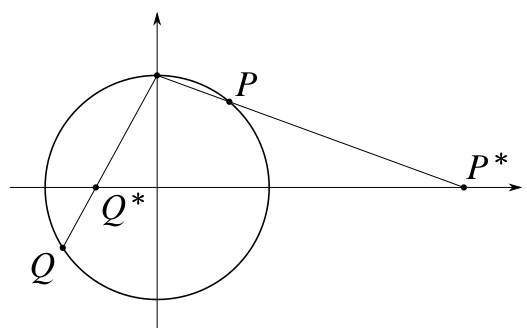
\includegraphics[scale=0.35]{projCirculo.png}
    \caption{Stereographic projection on 1-sphere case}
    \label{fig:projcirc}
\end{figure}

\section{3-sphere as a subset of the quaternions}
In here, we use the well known correspondence $(a,b,c,d) \in \R^4 \leftrightarrow a+bi+cj+dk \in \Hi$, and get:

\begin{equation*}
    S^{3} = \{a + bi+ cj + dk \in \Hi \cong \R^{4} : a^{2} + b^{2} + c^{2} + d^{2} = 1\}
\end{equation*}

\section{3-sphere as a matricial group}
%
%\subsection{1-sphere case}
%
%\begin{teorema}
%$S^{1} \cong SO(2)$
%\end{teorema}
%
%$SO(2) = \{ A \in M_{2x2}(\R) : A^{T}A = I$ and det(A) = 1 \}
%
%\begin{demonstracao}
%Firstly, note that
%\begin{gather*}
%    \psi: S^1 \rightarrow SO(2)\\
%    \psi(a+ib)=M_{a,b}=\begin{bmatrix}
%    a & -b\\
%    b & a
%    \end{bmatrix}
%\end{gather*}
%is a homomorphism.\\
%And since $z=a+ib \in S^1$ such that $\psi(z)=I$ %$\Rightarrow$ $a=1$ and $b=0$ $\Rightarrow z=1$,\\
%we have that $\psi$ is a monomorphism.\\
%
%Let A$=\begin{bmatrix}
%    a_{11} & a_{12}\\
%    a_{21} & a_{22}
%    \end{bmatrix} \in SO(2)$, we want $z$ in $S^1$
%\end{demonstracao}
%
%\subsection{3-sphere case}
%

Firstly, we'll define the special unitary group of degree 2:
\begin{equation*}
 SU(2) \doteq \{ A \in M_{2x2}(\C) : A^{*}A = AA^{*} = I \text{ and }|\det(A)| = 1 \}
\end{equation*}

\begin{teorema}
\begin{equation*}
    S^{3} \cong SU(2)
\end{equation*}
[Proof in appendix - proof \ref{proofTeoSU2}]
\end{teorema}

%%%%%%%%%%%%%%%%%%%%%%%%%%%%%%%%%%%%%%%%%%%%%%%%%%%%%%%%%%%%%%%%%%%%%%% proof
%%%%%%%%%%%%%%%%%%%%%%%%%%%%%%%%%%%%%%%%%%%%%%%%%%%%%%%%%%%%%%%%%%%%%%

\section{3-sphere as a union of circles (1-spheres) - Hopf fibration} %label?

We'll use here the correspondence 

\begin{equation*}
    a+bi+cj+dk \in \Hi \leftrightarrow (a+bi, c+di) \in \C^2.
\end{equation*}

So, $S^3$ can be written as 
\begin{equation*}
    S^3 = \{(a+bi, c+di) \in \C^2 : a^2+b^2+c^2+d^2=1\}
\end{equation*}

And then, we have:

\begin{equation*}
S^3 = \bigcup\limits_{q \in S^3} \{ e^{it}q : t \in \R \}
\end{equation*}
\begin{equation*}
= \bigcup\limits_{q \in S^3} \{ \lambda \cdot q \in \Hi : \lambda \in \C \} \cap S^3
\end{equation*}
\begin{equation*}
\cong \bigcup\limits_{(a+bi, c+di) \in S^3} \{ e^{it}(a+bi, c+di) \in \C^2 : t \in \R \}
\end{equation*}
\begin{equation}\label{direccoord}
     = \bigcup\limits_{(a+bi, c+di) \in S^3} \{ e^{it}(a+bi) \in \C : t \in \R \} \times \{ e^{it}(c+di) \in \C: t \in \R \}
\end{equation}

Note here that $|a+bi|^2 + |c+di|^2 = 1$
\\

The first equality is easy to prove:
\begin{equation*}
    \forall q \in S^3, q \in \{ e^{it}q : t \in \R \} 
\end{equation*}
\begin{equation*}
    \mbox{ and   } \forall t \in \R, \forall q \in S^3, ||e^{it}q||=||e^{it}|| \cdot ||q||=1\cdot1=1
\end{equation*}

The rest of them are trivial.

\begin{equation*}
\phi : \R \times S^3 \rightarrow S^3,
\end{equation*}
\begin{equation*}
\phi(t, q) = e^{it} \cdot q    
\end{equation*}
is a flow named Hopf flow. %pois

\begin{equation*}
\forall q \in S^3, \{ e^{it}q : t \in \R \},    
\end{equation*}
the Hopf flow orbit, is a simple closed curve and for different points in the 3-sphere, those sets are disjoint. %pois

\begin{equation*}
\forall q \in S^3, \{ \lambda \cdot q \in \Hi : \lambda \in \C \}    
\end{equation*}
is a 2-dimensional (real dimension) linear subspace and all points on
\begin{equation*}
\{ e^{it}q : t \in \R \}    
\end{equation*}
have distance 1 from the origin, therefore 
\begin{equation*}
\{ \lambda \cdot q \in \Hi : \lambda \in \C \} \cap S^3    
\end{equation*}
is a great circle in S$^3$.


\section{The 3-sphere as a union of tori}
Having seen the last section, it is easy to declare:

\begin{gather*}
S^3 = \bigcup\limits_{(z,w) \in S^3} \{ e^{it}z \in \C : t \in \R \} \times \{ e^{it}w \in \C: t \in \R \} \mbox{ with } |z|^2 + |w|^2 = 1 \\
= \bigcup\limits_{0 \leq r \leq 1} \bigcup \{\{ e^{it}z \in \C : t \in \R \} \times \{ e^{it}w \in \C: t \in \R \} : |z|^2 = r^2 \mbox{ and } |w|^2 = 1-r^2\} \\
= \bigcup\limits_{0 \leq r \leq 1} \{ z \in \C : |z| = r \} \times \{ w \in \C : |w| = \sqrt{1-r^2} \}. \\
\end{gather*}

\begin{equation*}
 \forall 0 \leq r \leq 1, \{ z \in \C : |z| = r \} \times \{ w \in \C : |w| = \sqrt{1-r^2} \}
\end{equation*}
is called Hopf torus.

If r = 0, 1; the Hopf torus will be a circle - a degenerate torus.
As r increases from 0 to 1, the torus will interpolate those circles, passing from tori much close to the circle of r = 0, to tori close to the one of r = 1.

Here, we can also easily note that for each 0 $<$ r $<$ 1, the Hopf torus is a disjoint union of Hopf circles:

\begin{equation*}
    \{ z \in \C : |z| = r \} \times \{ w \in \C : |w| = \sqrt{1-r^2} \}
\end{equation*}

\begin{equation*}
    = \bigcup\limits_{(a+bi,c+di) \in S^3, |a+bi|=r} \{ e^{it}(a+bi) \in \C : t \in \R \} \times \{ e^{it}(c+di) \in \C: t \in \R \}
\end{equation*}

\section{Those fibrations in $\R^3$}

%Beginning with the Hopf torus, we will prove that each one of them will be sent by the stereographic projection to a ring torus in $\R^3$, being the circle a degenerate torus.

Each Hopf torus will be sent by the stereographic projection to a ring torus in $\R^3$, being the circle a degenerate torus. And those ring tori are all concentric. [Proof in appendix - proof \ref{proofHopfStereo}]

\begin{figure}[H]
    \centering
    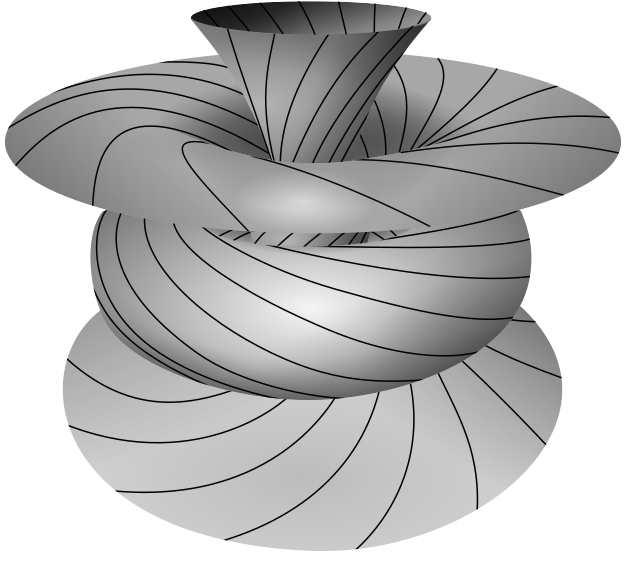
\includegraphics[scale=0.35]{torosHopf.png}
    \caption{The image by a stereographic projection of three non-degenerate Hopf tori (two of them are cut and the image of some Hopf circles is also drawn).}
    \label{fig:3}
\end{figure}

%%%%%%%%%%%%%%%%%%%%%%%%%%%%%%%%%%%%%%%%%%%%%%%%%%%%%%%%%%%%%%%%%%%%%%% proof
%%%%%%%%%%%%%%%%%%%%%%%%%%%%%%%%%%%%%%%%%%%%%%%%%%%%%%%%%%%%%%%%%%%%%%

Now about each Hopf circle, on equation \ref{direccoord}, one can note that any Hopf circle takes a turn in each of the coordinated directions of the Hopf torus in which it is. Consequently, the same will occur with their images by stereographic projection, remembering that every ring torus is homeomorphic to the cartesian product of two circles. Then, each Hopf circle will be sent to a Villarceau circle.

\begin{figure}[H]
    \centering
    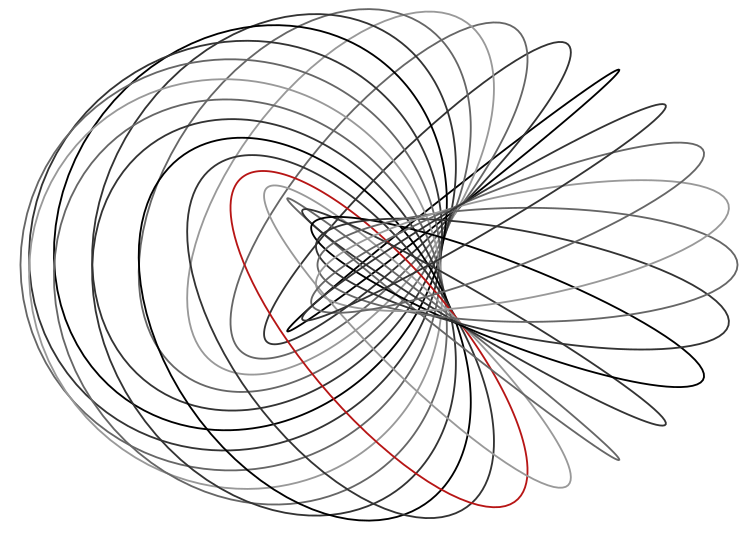
\includegraphics[scale=0.35]{toroHopf.png}
    \caption{Stereographic projection of some Hopf circles in the same Hopf torus.}
    \label{fig:toroHopf}
\end{figure}

\section{Villarceau circles}

Villarceau circles are the ones that "take a turn in each of the circles of the cartesian product form of the torus".\\
We'll show here that they exist and how they are.\\
Given a torus, if they exist, being circles, they would be 2 real dimensional, and since thay take a turn in each of the circles of the cartesian product form of the torus, would be given by the section of a torus along a diagonal plane bitangent that passes through the center of the torus. Taking this intersection, if it give us circles, will be the Villarceau circles. So let's put a coordinate system and prove that:\\

\begin{figure}[H]
    \centering
    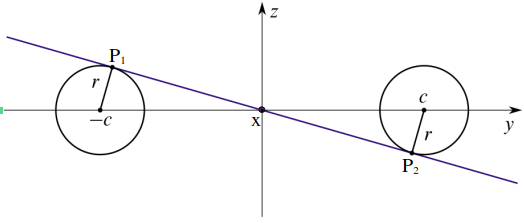
\includegraphics[scale=0.35]{villar.png}
    \caption{The central vertical section of the union of the plane and torus described above with the coordinates chosen. Imagine the hole figure with the torus being given by the rotation of these two circles around the z-axis and with the plane being the one that have the x-axis and the purple line.}
    \label{fig:villar}
\end{figure}

Equation of the torus:

\begin{gather*}
    (x^2+y^2+c^2-r^2)^2 = 4c^2(x^2+y^2)
\end{gather*}

Equation of the plane:

\begin{gather*}
    \sqrt{c^2-r^2}z+ry=0
\end{gather*}

So, the intersection of these figures will be given by the solution set A of:

\begin{gather*}
    \begin{cases}
        (x^2+y^2+c^2-r^2)^2 = 4c^2(x^2+y^2)\\
        \sqrt{c^2-r^2}z+ry=0
    \end{cases}
\end{gather*}

But since

\begin{gather*}
    (x^2+y^2+c^2-r^2)^2 = 4c^2(x^2+y^2) \Leftrightarrow (x^2+y^2+r^2-c^2)^2 - 4r^2x^2 = 4r^2y^2 - 4(c^2-r^2)z^2
\end{gather*}

We have:

\begin{gather*}
    \begin{cases}
        (x^2+y^2+c^2-r^2)^2 = 4c^2(x^2+y^2)\\
        \sqrt{c^2-r^2}z+ry=0
    \end{cases}
    \Leftrightarrow
    \begin{cases}
        \sqrt{c^2-r^2}z+ry=0\\
        (x^2+y^2+r^2-c^2)^2 - 4r^2x^2 = 4r^2y^2 - 4(c^2-r^2)z^2 = 0
    \end{cases}\\
    \Leftrightarrow
    \begin{cases}
        \sqrt{c^2-r^2}z+ry=0\\
        (x^2+y^+z^2+r^2-c^2+2rx)(x^2+y^2+z^2+r^2-c^2-2rx) = 0
    \end{cases}
    \Leftrightarrow\\
    \begin{cases}
        \sqrt{c^2-r^2}z+ry=0\\
        ((x+r)^2+y^2+z^2-c^2)((x-r)^2+y^2+z^2-c^2) = 0
    \end{cases}
\end{gather*}

And then, $A = A_1 \cup A_2$, being
\begin{gather*}
    A_1 \text{ the solution set of } \alpha_1 = 
    \begin{cases}
        \sqrt{c^2-r^2}z+ry=0\\
        (x+r)^2+y^2+z^2-c^2 = 0 \text{ (*)}
    \end{cases}\\
    \text{and } A_2 \text{ the solution set of } \alpha_2 = 
    \begin{cases}
        \sqrt{c^2-r^2}z+ry=0\\
        (x-r)^2+y^2+z^2-c^2 = 0 \text{ (**)}
    \end{cases}
\end{gather*}

Since (*) and (**) are equations of different 2-spheres and $P_1$ and $P_2$ are different points that are in $A_1$ and $A_2$ (the non-empty intersection of a sphere with a plane is either a single point, or a circle), we have that A is the union of two circles $A_1$ and $A_2$, both with radius $c$ and enteirely on the initial plane, but $A_1$ with center $(-r, 0, 0)$ and $A_2$ centered on $(r, 0, 0)$, the just proved Villarceau circles in this imposed coordinate system.
%\section{3-sphere as two solid tori}
%
%\begin{figure}[H]
%    \centering
%    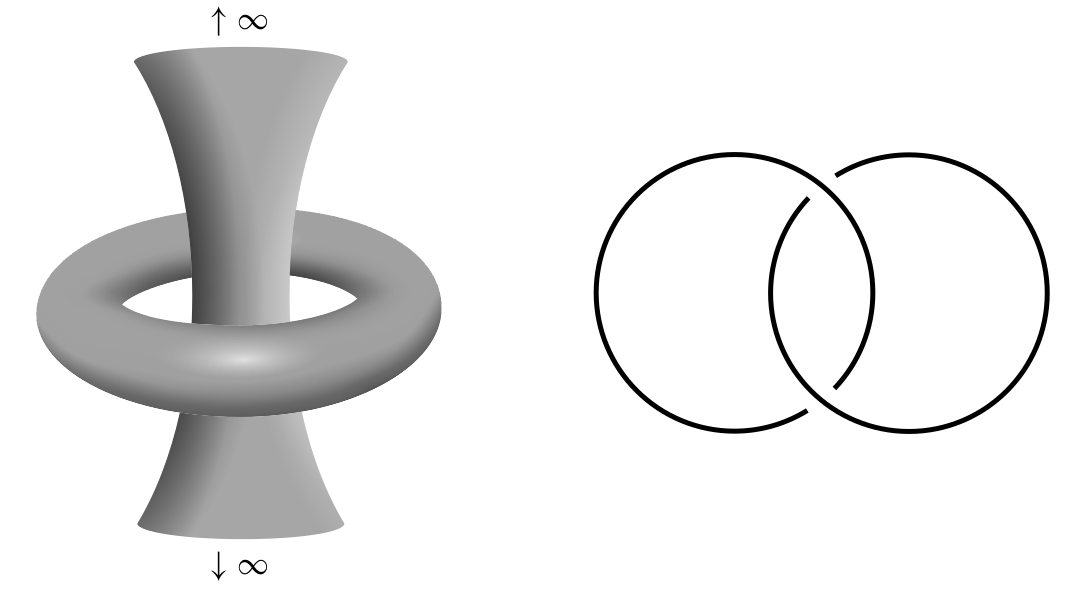
\includegraphics[scale=0.35]{torosSolid.png}
%    \caption{}
%    \label{fig:0}
%\end{figure}
%
%\section{3-sphere as a Lie group}
%
%SU(2) $\cong$ S$^3$ is an example of a Lie group, a group, which we know that SU(2) is, that is also a smooth manifold, which we know that S$^3$ is.
%
%The related Lie algebra will be \textswab{SU}(2) = $\{ ui + vj + wk \in \Hi : u, v, w \in \R\}$.

\chapter{Activity plan for the next period}\label{chp:plano}

In the final part of this project, we aim to do a deep study of some of the main methods of exponential integration for problems in dynamic systems, with emphasis on the paper \cite{Hochbruck2010}.

Here, the undergraduate will study the construction, analysis, implementation and application of them and at the end, it is expected that she is familiar with modern techniques of numerical methods.

Specific goals:

\begin{itemize}
    \item Study the review para of Hochbruck and Ostermann \cite{Hochbruck2010} on numerical exponential integrators.
    \item Look into the main convergence theorems for exponential integration, based on references contained in Hochbruck and Ostermann \cite{Hochbruck2010}.
    \item Implement some idealized examples from the reference, looking into matrix exponential methods from Moler and Van Loan \cite{Moler2003}.
    \item Implement an exponential integration scheme for a 1D wave problem, possibly aiming at application to atmospheric waves.
\end{itemize}

This work is intended to be developed in collaboration between the FAPESP Thematic project on Dynamical Systems, led by the supervisor of this current proposal, André Salles de Carvalho, process 16/25053-8, and the FAPESP Young Investigator project on Numerical Methods, process 21/06176-0, led by a collaborator of this current proposal, Pedro S. Peixoto.

\chapter{Participation in scientific event, list of publications and list of papers prepared or submitted}\label{chp:participacao}

Nothing to declare.

%\chapter{Participation in scientific event}\label{chp:participacao}

Nothing to declare.

%\begin{itemize}
%    \item Palestra sobre Emmy Noether;
%    \item Palestra sobre 
%    \item Palestra sobre A forma do Universo e a Matemática;
%    \item Palestra Luz, câmera, ação (de grupos na esfera);
%    \item Curso de verão de introdução à dinâmica complexa - IMPA;
%    \item Workshop mulheres na matemática;
%    \item Minicurso espaços hiperbólicos.
%\end{itemize}

%\chapter{List of publications}\label{chp:publicacoes}

Nothing to declare.

%\chapter{List of papers prepared or submitted}\label{chp:trabalhos}

Nothing to declare.

\addcontentsline{toc}{chapter}{\bibname}
\bibliographystyle{abntex2-num}
\bibliography{bibliografia}

\chapter{Appendix}\label{chp:apendices}

\section{Proof \ref{proofRemark3}}

\begin{proof} \label{proofRemark3}
For the demonstration, we'll use the results from Ahlfors (page 20 of \cite{Ahlfors}Ahlfors's book - exercise 1 and equation (28)):

\begin{gather*}
d(\mbox{g}^{-1}(z), \mbox{g}^{-1}(z')) = \frac{2|z-z'|}{\sqrt{(1+|z|^2)(1+|z'|^2)}}
\end{gather*}
being $d$ the distance in $\R^3$.

"$pp'=-1 \Leftrightarrow $ g$^{-1}(p)$ and g$^{-1}(p')$ are diametrically opposite points on $S^2$." ($\bigstar$)

\noindent($\Rightarrow$)

Let A and B be the poles of the rotation R of $S^2$.

Let's call $a$ = g(A) and $-\frac{1}{a}$=g(B) (it is possible because of ($\bigstar$)).

And let them be the foci of the circles in C$_2$, then $\frac{|z-a|}{|z+\frac{1}{a}|}$ is a complex constant $\forall z$ in every circle in C$_2$, let's call it $c$.

Let Z = g$^{-1}(z)$,

Then, we have:
\begin{gather*}
    \frac{||Z-A||}{||Z-B||}=\frac{\frac{2|z-a|}{\sqrt{(1+|z|^2)(1+|a|^2)}}}{\frac{2\left|z+\frac{1}{a}\right|}{\sqrt{(1+|z|^2)\left(1+\left|-\frac{1}{a}\right|^2\right)}}}=\frac{|z-a|}{\left|z+\frac{1}{a}\right|} \sqrt{\frac{1+\left|-\frac{1}{a}\right|^2}{1+|a|^2}}=c\sqrt{\frac{1+\left|-\frac{1}{a}\right|^2}{1+|a|^2}} = c' \in \C
\end{gather*}
Since $a$ is fixed, we could call
\begin{equation*}
c\sqrt{\frac{1+\left|-\frac{1}{a}\right|^2}{1+|a|^2}}    
\end{equation*}
a constant ($c'$).

Knowing that the stereographic projection is always a restriction of an inversion, and that inversion has order 2, it is clear that g$^{-1}[\alpha_2]$ is a circle on S$^2$, $\forall \alpha_2 \in$ C$_2$. More precisely, because of the last equation, is a circle on a plane perpendicular to the axis that passes through A and B, that we know that are diametrically opposite points on $S^2$ because of $(\bigstar)$. So, since R can't change them, g $\circ$ R $\circ$ g$^{-1}$ can't alter the circles on C$_2$, and therefore, is an elliptic transformation and its fixed points are $a$ and $-\frac{1}{a}$.

\noindent($\Leftarrow$)

g $\circ$ R $\circ$ g$^{-1}$ is an elliptic transformation with fixed points $a$ and $-\frac{1}{a}$, be C$_1$ and C$_2$ the expected families with foci $a$ and $-\frac{1}{a}$, so g $\circ$ R $\circ$ g$^{-1}$ carries each circle of C$_2$ in itself and each circle of C$_1$ in another circle in C$_1$ with fixed angle between them (independant on the choice of the first circle in C$_1$), let's call it $\theta$.

Since inversions are conformal, so is g and g$^{-1}$. And therefore, we know that R don't alter g$^{-1}[\alpha_2]$, g$^{-1}(a)$ nor g$^{-1}\left(-\frac{1}{a}\right)$, $\forall \alpha_2 \in$ C$_2$, the last two of them being antipodal points on S$^2$ ($\bigstar$), and that R rotates the pre-image by g of the circles of C$_1$ by $\theta$. Note here that since g$^{-1}$ carries circles into circles, it will carry the circles that pass through $a$ and $-\frac{1}{a}$ (the circles in C$_1$) to circles that pass through g$^{-1}(a)$ and g$^{-1}\left(-\frac{1}{a}\right)$, since those are antipodals, g$^{-1}$[C$_1$] covers S$^2$ with maximal circles that pass through those two points (like the longitudinal lines on Earth), and that's why we can tell that R rotates the pre-image by g of the circles of C$_1$ by $\theta$.

So, R is a rotation on S$^2$.
\end{proof}

%%%%%%%%%%%%%%%%%%%%%%%%%%%%%%%%%%%%%%%%%%%%%%%%%%%%%%%%%%%%%%%%%%%%%%

\section{Proof \ref{proofTeoSU2}}

\begin{proof} \label{proofTeoSU2}
We'll use here the matrix form of quaternions:
\begin{gather*}
    a+bi+cj+dk \leftrightarrow  M_{a+bi,c+di}=\begin{bmatrix}
    a+ib & -c-di\\
    c-di & a-bi
    \end{bmatrix}
\end{gather*}
And it is clear that:
\begin{equation*}
    ||q||=1 \Leftrightarrow det(M_{a+bi,c+di})=1
\end{equation*}

\begin{equation*}
    M_{a+bi,c+di}^{*}M_{a+bi,c+di}=I \Leftrightarrow a^2+b^2+c^2+d^2=1
\end{equation*}
Thus, we obtain the homomorphism of groups:
\begin{gather*}
    \psi: S^3 \rightarrow SU(2)\\
    \psi(a+bi+cj+dk) = M_{a+bi,c+di}
\end{gather*}
Let's show that $\psi$ is an isomorphism.

In fact, $\psi$ is injective, because 

\begin{equation*}
    M_{a+bi,c+di} = \begin{bmatrix}
    a+ib & -c-di\\
    c-di & a-bi
    \end{bmatrix} = I \Rightarrow a=1, b=c=d=0.
\end{equation*}
    
And is surjective:
\begin{gather*}
    \forall A=\begin{bmatrix}
    z_{11} & z_{12}\\
    z_{21} & z_{22}
    \end{bmatrix} \in SU(2)
\end{gather*}

We denote $v_1 = 
\begin{bmatrix}
    z_{11}\\
    z_{21} 
\end{bmatrix} $
and $v_2 = 
\begin{bmatrix}
    z_{12}\\
    z_{22}
\end{bmatrix}$

\begin{gather*}
    A^{*}A = \begin{bmatrix}
    \bar{z}_{11} & \bar{z}_{21}\\
    \bar{z}_{12} & \bar{z}_{22}
    \end{bmatrix} \cdot \begin{bmatrix}
    z_{11} & z_{12}\\
    z_{21} & z_{22}
    \end{bmatrix} = \begin{bmatrix}
    \langle v_1 \; , \; v_1 \rangle & \langle v_2 \; , \; v_1 \rangle\\
    \langle v_1 \; , \; v_2 \rangle & \langle v_2 \; , \; v_2 \rangle
    \end{bmatrix} = \begin{bmatrix}
    1 & 0\\
    0 & 1
    \end{bmatrix} = I
\end{gather*}

Since $\langle v_1 \; , \; v_2 \rangle = 0$, 
\begin{gather*}
    v_2 \in v_1^{\perp} = \left\{\begin{bmatrix}
    z\\
    w
    \end{bmatrix} : \left\langle v_1 \; , \; \begin{bmatrix}
    z\\
    w
    \end{bmatrix} \right\rangle = 0 \right\}
\end{gather*}

But
\begin{align*}
    z_{11}\bar{z}+z_{21}\bar{w}=0 \Leftrightarrow \bar{z}=-\frac{z_{21}}{z_{11}}\bar{w} \Leftrightarrow z=-\frac{\bar{z}_{21}}{\bar{z}_{11}}w
\end{align*}

So, 
\begin{gather*}
    v_2 \in v_1^{\perp} = \left\{ w\begin{bmatrix}
    -\frac{\bar{z}_{21}}{\bar{z}_{11}}\\
    1
    \end{bmatrix} : w \in \C \right\}
\end{gather*}


Beside that, $\langle v_2 \; , \; v_2 \rangle = 1$.
But,
\begin{gather*}
    1 = \left\langle w\begin{bmatrix}
    -\frac{\bar{z}_{21}}{\bar{z}_{11}}\\
    1
    \end{bmatrix} \; , \; w\begin{bmatrix}
    -\frac{\bar{z}_{21}}{\bar{z}_{11}}\\
    1
    \end{bmatrix} \right\rangle = |w|^2 \left(\frac{|\bar{z}_{21}|^2}{|\bar{z}_{11}|^2}+1\right)
\end{gather*}

So,
\begin{gather*}
    |w| = \frac{|z_{11}|}{\sqrt{|z_{21}|^2 + |z_{11}|^2}} = |z_{11}|
\end{gather*}

because $\langle v_1 \; , \; v_1 \rangle = 1$.

And also 
\begin{equation*}
    \det(A)=z_{11}z_{22}-z_{12}z_{21}=1.
\end{equation*}

Then,
\begin{gather*}
    1 = z_{11}w-z_{21}(-)\frac{\bar{z}_{21}}{\bar{z}_{11}}w = w \left( z_{11}+\frac{|{z}_{21}|^2}{\bar{z}_{11}} \right) = w \left( \frac{|{z}_{11}|^2+|{z}_{21}|^2}{\bar{z}_{11}} \right) = \frac{w}{\bar{z}_{11}}
\end{gather*}

since $\langle v_1 \; , \; v_1 \rangle = 1$.

So, $w = \bar{z}_{11}$

Thus,
\begin{gather*}
    v_2 = \bar{z}_{11} \begin{bmatrix}
    -\frac{\bar{z}_{21}}{\bar{z}_{11}}\\
    1
    \end{bmatrix} = \begin{bmatrix}
    -\bar{z}_{21}\\
    \bar{z}_{11}
    \end{bmatrix}\\
    A = \begin{bmatrix}
    z_{11} & -\bar{z}_{21}\\
    z_{21} & \bar{z}_{11}
    \end{bmatrix}
\end{gather*}

And therefore, if we take 
\begin{equation*}
q_{A} = \Re(z_{11}) + \Im(z_{11})i + \Re(z_{21})j - \Im(z_{21})k,
\end{equation*}
it is obvious that $||q_{A}||=1$ and $\psi (q_{A}) = A$, concluding our demonstration that $\psi$ is a isomorphism. 
\end{proof}

%%%%%%%%%%%%%%%%%%%%%%%%%%%%%%%%%%%%%%%%%%%%%%%%%%%%%%%%%%%%%%%%%%%%%%

\section{Proof \ref{proofghomeo}}

\begin{proof} \label{proofghomeo}
g is continuous because, for $(\vec{x},t)\neq(0, ..., 0, 1)$ it is a well defined fraction of polynomial functions and 
\begin{equation*}
    \operatorname{g}(\vec{x}, t) \rightarrow \infty \text{ as }(\vec{x},t) \rightarrow (0, ..., 0, 1)
\end{equation*}
since is a product of a limited term by a term going to $\infty$.\\
Surjective because $\forall \hat{x} \in \hat{\R}^n$,
\begin{equation*}
    \left(\frac{2\hat{x}}{||\hat{x}||^2+1},\frac{||\hat{x}||^2-1}{||\hat{x}||^2+1}\right) \in S^n,
\end{equation*}
and
\begin{equation*}
\operatorname{g}\left(\frac{2\hat{x}}{||\hat{x}||^2+1},\frac{||\hat{x}||^2-1}{||\hat{x}||^2+1}\right) = \hat{x}.
\end{equation*}

g is injective because, if t and $\tilde{t} \neq$ 1.
\begin{equation*}
\frac{1}{1 - t} \vec{x} =  \frac{1}{1 - \tilde{t}} \tilde{x} \Rightarrow    
\end{equation*}
\begin{equation*}
\vec{x} =  \frac{1 - t}{1 - \tilde{t}} \tilde{x} \Rightarrow 
\end{equation*}
\begin{equation*}
    ||\vec{x}||^2 + t^2 =  \frac{(1 - t)^2}{(1 - \tilde{t})^2}||\tilde{x}||^2 + t^2 = ||\tilde{x}||^2 + \tilde{t}^2 = 1 \Rightarrow
\end{equation*}
\begin{equation*}
   t = \tilde{t}; \frac{1}{1 - t} \vec{x} =  \frac{1}{1 - \tilde{t}} \tilde{x} \Rightarrow 
\end{equation*}
\begin{equation*}
    t = \tilde{t}; \vec{x} = \tilde{x} \Rightarrow
\end{equation*}
\begin{equation*}
    (\vec{x},t) = (\tilde{x}, \tilde{t})
\end{equation*}
And if not, the point will be $(0, ..., 0, 1)$, for which there is a 1 to 1 correspondence.

\begin{gather*}
\operatorname{g}^{-1} : \hat{\R}^n \rightarrow S^n \\
\operatorname{g}^{-1}(\vec{u}) =
    \begin{cases}
        (0, ..., 0, 1), \text{ if } \vec{u} = \infty \\
        \left( \frac{2\vec{u}}{||\vec{u}||^2+1}, \frac{||\vec{u}||^2-1}{||\vec{u}||^2+1} \right), \mbox{ } c.c.
    \end{cases}
\end{gather*}

g$^{-1}$ is continuous.

For $\vec{u}\neq \infty$, it is because norm and algebra of continuous functions are continuous functions.

In $\infty$, let $(a_n)_n$ be a sequence in $\hat{\R}^n$ converging to $\infty$,
\begin{equation*}
\operatorname{g}^{-1}(a_n) = \left( \frac{2a_n}{||a_n||^2+1}, \frac{||a_n||^2-1}{||a_n||^2+1} \right) = \left( \frac{2 \frac{a_n}{||a_n||^2}}{1 + \frac{1}{||a_n||^2}}, \frac{1-\frac{1}{||a_n||^2}}{1+\frac{1}{||a_n||^2}} \right)
\end{equation*}
\begin{equation*}
 \rightarrow \left( \frac{2}{\infty}, ..., \frac{2}{\infty}, \frac{1-\frac{1}{\infty^2}}{1+\frac{1}{\infty^2}} \right) = \left( 0, ..., 0, \frac{1-0}{1+0} \right) = (0, ..., 0, 1) \text{ as }n \rightarrow \infty    
\end{equation*}

This ends the proof that g is a homeomorphism.
\end{proof}

%%%%%%%%%%%%%%%%%%%%%%%%%%%%%%%%%%%%%%%%%%%%%%%%%%%%%%%%%%%%%%%%%%%%%%

\section{Proof \ref{proofHopfStereo}}

\begin{proof} \label{proofHopfStereo}
Fix 0$<$r$<$1 and let T$_{r}$ be the relative Hopf circle:
\begin{equation*}
\{a+bi \in \C : a^2+b^2 = r^2 \} \times \{c+di \in \C : c^2+d^2 = 1 - r^2 \},    
\end{equation*}
which is isomorphic to 
\begin{equation*}
    \{(a,b) \in \R^2 : a^2+b^2 = r^2 \} \times \{(c,d) \in \R^2 : c^2+d^2 = 1 - r^2 \} 
\end{equation*}
\begin{equation*}
    = \{(a,b,c,d) \in \R^4 : a^2+b^2 = r^2\mbox{ and }c^2+d^2 = 1 - r^2\}.
\end{equation*}

\begin{equation*}
    \mbox{Let } K_{r} \mbox{ be }T_{r} \cap \R^3_{(x,z,t)},
\end{equation*}

\begin{equation*}
    \mbox{where }\R^3_{(x,z,t)} = \{(x,y,z,t) \in \R^4 : y=0\}.
\end{equation*}


\begin{equation*}
\mbox{So }K_{r} = \{(x,y,z,t) \in \R^4 : y=0, x^2=r^2, z^2+t^2 = 1-r^2\}    
\end{equation*}
\begin{equation*}
    = S^2_{(x,z,t)} \cap \{(x,y,z,t) \in \R^4 : y=0, x=\pm r \},
\end{equation*}

\begin{equation*}
\mbox{being }S^2_{(x,z,t)} = {(x,y,z,t) \in \R^4 : y=0, x^2+z^2+t^2=1}, 
\end{equation*}
the 2-sphere in $\R^3_{(x,z,t)}$. 

\begin{figure}[H]
    \centering
    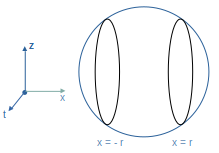
\includegraphics[scale=0.75]{Kr.png}
    \caption{$K_{r}$ in black.}
    \label{fig:Kr}
\end{figure}



Moreover, 
\begin{equation*}
\mbox{let }A_\theta = \begin{bmatrix}
\cos\theta & -\sin\theta & 0\\
\sin\theta & \cos\theta & 0\\
0 & 0 & 1
\end{bmatrix},    
\end{equation*}
 the rotation around the third coordinate and
 
\begin{equation*}
A'_\theta = \begin{bmatrix}
\cos\theta & -\sin\theta & 0 & 0\\
\sin\theta & \cos\theta & 0 & 0\\
0 & 0 & 1 & 0\\
0 & 0 & 0 & 1
\end{bmatrix},
\end{equation*}
the rotation "around the two last coordinates" which are classic examples of orthogonal matrices.

Besides that, we will call g the stereographic projection:

\begin{gather*}
\operatorname{g} : S^3 \rightarrow \hat{\R}^3 \\
\operatorname{g}(x_1, x_2, x_3, t) =
    \begin{cases}
        \infty, \text{ if } x_1 = x_2 = x_3 = 0, t = 1 \\
        \frac{1}{1 - t} (x_1, x_2, x_3), \mbox{ } c.c.
    \end{cases}
\end{gather*}

and

\begin{gather*}
\operatorname{g}_{(x,z,t)} = \restr{\operatorname{g}}{S^2_{(x,z,t)}}: S^2_{(x,z,t)} \rightarrow \R^3
\\
    \operatorname{g}_{(x,z,t)}(x, 0, z, t) =
    \begin{cases}
        \infty, \text{ if } x = z = 0, t = 1 \\
        \frac{1}{1 - t} (x, 0, z), \mbox{ } c.c.
    \end{cases}
\end{gather*}

Here we can easily see that g$_{(x,z,t)}$ is the stereographic projection sending the 2-sphere S$^2_{(x,z,t)}$ to the 2-plane 
\begin{equation*}
    \{(x,y,z) \in \R^4 : y = 0 \}.
\end{equation*}

And then, since K$_{r}$ is on S$^2_{(x,z,t)}$, we can define
\begin{equation*}
\famcirc_{r} := \operatorname{g}_{(x,z,t)}[K_{r}],    
\end{equation*}
being the stereographic projection acting on two symmetrical vertical circles on the 2-sphere, will be two Apollonian circles on the xz-plane of $\R^3$ [See the section \ref{TLF}], symmetric in relation to the $z$ axis, as you can see on figure \ref{fig:oi}. %não tenho certeza se era esse o nome do círculo ou da rede%

\begin{figure}[H]
    \centering
    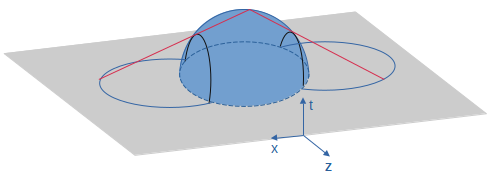
\includegraphics[scale=0.35]{projest.png}
    \caption{An illustration of $\operatorname{g}_{(x,z,t)}$, represented by the pink lines, with $K_{r}$ in black.}
    \label{fig:oi}
\end{figure}

And we can see that, $\forall (x,y,z,t) \in S^3,$
\begin{equation*}
    A_{\theta} \circ \operatorname{g}(x,y,z,t) = A_{\theta} \left(\frac{1}{1-t}(x,y,z)\right)
\end{equation*}
\begin{equation*}
    = \frac{1}{1-t} A_{\theta}(x,y,z)
\end{equation*}
\begin{equation*}
    = \operatorname{g}(A_{\theta}(x,y,z),t)
\end{equation*}
\begin{equation*}
    = \operatorname{g}\circ A'_{\theta}(x,y,z,t) 
\end{equation*}

noting that $(A_{\theta}(x,y,z),t)$ is in the domain of $g$, i.e. $(A_{\theta}(x,y,z),t) \in S^3$ because:
\begin{equation*}
    ||(A_{\theta}(x,y,z),t)||^2 = ||A_{\theta}(x,y,z)||^2 + t^2 = \langle A_{\theta}(x,y,z) \; , \; A_{\theta}(x,y,z) \rangle + t^2 
\end{equation*}
\begin{equation*}
    = \langle (x,y,z) \; , \; (x,y,z) \rangle + t^2 = x^2 + y^2 + z^2 + t^2 = 1
\end{equation*}

since $(x,y,z,t) \in S^3$ and $A_{\theta}$ is an orthogonal matrix.

With all this, we have:

\begin{equation*}
    \operatorname{g} \circ A'_{\theta}[K_{r}] = A_{\theta} \circ \operatorname{g}[K_{r}] = A_{\theta} \circ \operatorname{g}_{(x,z,t)}[K_{r}] = A_{\theta}[\famcirc_{r}]
\end{equation*}

And then:

\begin{equation*}
    \bigcup\limits_{0 \leq \theta \leq 2\pi} A_{\theta}[\famcirc_{r}] = \bigcup\limits_{0 \leq \theta \leq 2\pi} \operatorname{g} \circ A'_{\theta}[K_{r}] = \operatorname{g}\left(\bigcup\limits_{0 \leq \theta \leq 2\pi} A'_{\theta}[K_{r}]\right)
\end{equation*}

But C$_{r}$ is two circles on 
\begin{equation*}
\{(x,y,z) \in \R^3 : y = 0\},    
\end{equation*}
symmetric in relation to the $z$ axis, so the union of all the rotations around the $z$ axis 
\begin{equation*}
    \left(\bigcup\limits_{0 \leq \theta \leq 2\pi} A_{\theta}[\famcirc_{r}]\right)
\end{equation*}
will give us a ring torus in $\R^3$.

And:
\begin{equation*}
\bigcup\limits_{0 \leq \theta \leq 2\pi} A'_{\theta}[K_{r}] = T_{r} = \{(a,b,c,d) \in \R^4 : a^2+b^2=r^2 \mbox{ and } c^2+d^2=1-r^2\},
\end{equation*}
remembering that
\begin{equation*}
    K_{r} = \{(x,y,z,t) \in \R^4 : y=0, x^2=r^2, z^2+t^2 = 1-r^2\}:
\end{equation*}
$\subseteq$ : $\forall (x,0,z,t) \in K_{r}, \forall \theta \in [0,2\pi]$,
\begin{equation*}
    A'_{\theta}(x,0,z,t) = (x \cos\theta, x \sin{\theta}, z, t) \mbox{ with } x^2 = r^2 \mbox{ and } z^2+t^2=1-r^2.
\end{equation*}
\begin{equation*}
\mbox{ Since } (x \cos\theta)^2+(x \sin\theta)^2=x^2=r^2 \mbox{ and } z^2+t^2=1-r^2, A'_{\theta}(x,0,z,t) \in T_{r}.
\end{equation*}
$\supseteq$ : $\forall (x,y,z,t) \in T_{r}$,\\
\begin{equation*}
    \mbox{ we have } x^2+y^2=r^2 \mbox{ and } z^2+t^2=1-r^2,
\end{equation*}
\begin{equation*}
\mbox{ let } \hat{\theta} \mbox{ be } \arccos\left(\frac{x}{r}\right), \mbox{ so } \sin \hat{\theta} = \frac{y}{r}.    
\end{equation*}
\begin{equation*}
\mbox{ Therefore, }  (x,y,z,t) = (r \cos\hat{\theta}, r \sin\hat{\theta}, z, t) = A_{\hat{\theta}}(r,0,z,t).
\end{equation*}
\begin{equation*}
\mbox{ Since } z^2+t^2=1-r^2, (r,0,z,t) \in K_{r}, \mbox{ therefore } (x,y,z,t) \in A_{\hat{\theta}}(K_{r})
\end{equation*}

For r = 0, 1; we already know that the image will be a circle since the stereographic projection, being basically a restriction of a inversion, sends a circle in a circle.

But the same previous demonstration can be applied, with
\begin{equation*}
T_0=\{(x,y,z,t) \in \R^4 : x=y=0, z^2+t^2=1\},    
\end{equation*}
\begin{equation*}
T_1=\{(x,y,z,t) \in \R^4 : z=t=0, x^2+y^2=1\}    
\end{equation*}
so 
\begin{equation*}
    K_0=T_0 \subseteq \R^3_{(x,z,t)},
\end{equation*}
\begin{equation*}
    K_1=\{(-1,0,0,0),(1,0,0,0)\}
\end{equation*}
note that $K_1$ is the 2 foci of the Apollonian family of circles,

\begin{figure}[H]
    \centering
    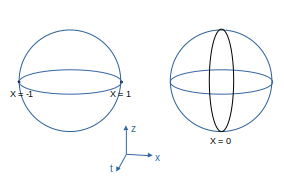
\includegraphics[scale=0.50]{K0K1.png}
    \caption{In black, $K_1$ on the left and $K_0$ on the right.}
    \label{fig:K0K1}
\end{figure}

so
 \begin{equation*}
    \famcirc_0=\{(x,z,t) \in \R^3 : x=t=0\}, 
 \end{equation*}
 \begin{equation*}
    \famcirc_1=\{(-1,0,0); (1,0,0)\}, 
 \end{equation*}
 notable cases of the stereographic projection,
 
 \begin{figure}[H]
    \centering
    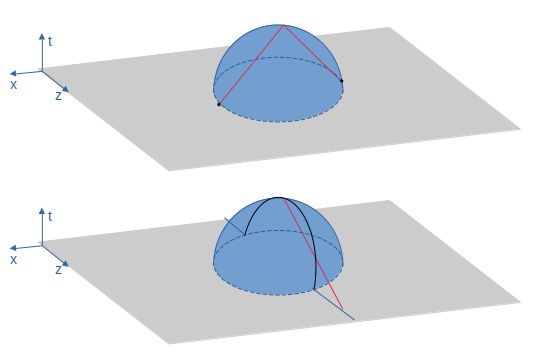
\includegraphics[scale=0.50]{C0C1.png}
    \caption{Above, $\famcirc_1$, and below, $\famcirc_0$ being "constructed" by the stereographic projection.}
    \label{fig:C0C1}
\end{figure}
 
 and then
 \begin{equation*}
 \operatorname{g}[T_0]=\famcirc_0
 \end{equation*}
 \begin{equation*}
 \operatorname{g}[T_1]=\{(x,z,t) \in \R^3 : z=0, x^2+t^2=1\},
 \end{equation*}
 circles on $\R^3$, being the line a circle that passes through infinity.

\begin{figure}[H]
    \centering
    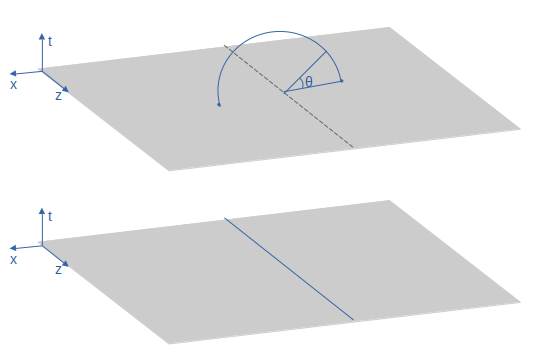
\includegraphics[scale=0.50]{gC0gC1.png}
    \caption{Above, g$[T_1]$ being "constructed" by union of rotations of C$_1$, and below, g$[T_0]$.}
    \label{fig:gC0gC1}
\end{figure}

In conclusion, each Hopf torus is sent to a ring torus in $\R^3$ by the stereographic projection, and the decomposition of $S^3$ in Hopf tori is sent to a union of all the rotations of the decomposition of the plane in Apollonian circles.
\end{proof}

\end{document}
